\documentclass[12pt, twoside]{article}
\usepackage[letterpaper, margin=1in, headsep=0.5in]{geometry}
\usepackage[english]{babel}
\usepackage[utf8]{inputenc}
\usepackage{amsmath}
\usepackage{amsfonts}
\usepackage{amssymb}
\usepackage{tikz}
\usetikzlibrary{quotes, angles}
\usepackage{graphicx}
\usepackage{enumitem}
\usepackage{multicol}

\newif\ifmeta
\metatrue %print standards and topics tags

\title{IB Math Applications and Interpretations}
\author{Chris Huson}
\date{March 2022}

\usepackage{fancyhdr}
\pagestyle{fancy}
\fancyhf{}
\renewcommand{\headrulewidth}{0pt} % disable the underline of the header
\raggedbottom

\fancyhead[LE]{\thepage}
\fancyhead[RO]{\thepage \\ Name: \hspace{4cm} \,\\}
\fancyhead[LO]{BECA / IB Math 6 Geometry \\* 16 March 2022}

\begin{document}
\subsubsection*{6.2 Right triangle trigonometry}
Do Now (PreQuiz)
\begin{enumerate}
\item Calculate each value. Round to the nearest thousandth.
  \begin{enumerate}
    \begin{multicols}{2}
    \item $\displaystyle \sin 19^\circ$ \vspace{1cm}
    \item $\displaystyle \cos 53^\circ$
    \item $\displaystyle \tan 39^\circ$ \vspace{1cm}
    \item $\displaystyle \sin 30^\circ$
    \end{multicols}
  \end{enumerate}
  \vspace{1cm}

\item Find $\theta$. Round to the nearest whole degree.
  \begin{enumerate}
    \begin{multicols}{2}
    \item $\displaystyle \theta = \sin^{-1} (\frac{3}{10})$ \vspace{1cm}
    \item $\displaystyle \theta = \tan^{-1} (1.50)$
    \item $\displaystyle \theta = \cos^{-1} (0.707)$ \vspace{1cm}
    \item $\displaystyle \tan \theta = \frac{2.6}{4.9}$
    \end{multicols}
  \end{enumerate} \vspace{2cm}

\item Solve each equation for $x$, rounding to the nearest tenth.
  \begin{enumerate}
    \begin{multicols}{2}
    \item $\displaystyle \cos 33^\circ = \frac{x}{21}$ \vspace{5cm}
    \item $\displaystyle \tan 16^\circ = \frac{3.7}{x}$
    \end{multicols}
  \end{enumerate}
  \vspace{3cm}

\item Given right $\triangle ABC$ with $AC=10$, $m\angle A=40^\circ$. Find the value of $BC=x$.
  \begin{flushright}
    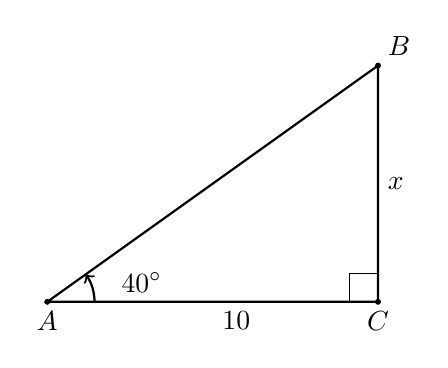
\begin{tikzpicture}[scale=0.6]
      \draw [thick](-1,0)--(6,0)--(6,5)--cycle;
      \draw [fill] (-1,0) circle [radius=0.05] node[below]{$A$};
      \draw [fill] (6,0) circle [radius=0.05] node[below]{$C$};
      \draw [fill] (6,5) circle [radius=0.05] node[above right]{$B$};
      \draw (6,0)++(-0.6,0)--++(0,0.6)--+(0.6,0);
      \node at (3,0)[below]{$10$};
      \node at (6,2.5)[right]{$x$};
      \draw [thick, ->] (0,0) arc [start angle=0, end angle=35.5, radius=1];
      \node at (1,0)[above]{$40^\circ$};
    \end{tikzpicture}
  \end{flushright}

  \newpage
  \item Graph and label $\triangle ABC$ with $A(0,0)$, $B(5,3)$, and $C(5,0)$. Calculate the length of each side of the triangle.
  \begin{enumerate}[itemsep=1.25cm]  
  \begin{multicols}{2}
        \item $AC=$
        \item $BC=$
        \item For the hypotenuse express the length as a radical.\\[0.25cm]
        (hint: use the Pythagorean theorem $a^2+b^2=c^2$)\\[0.25cm]
        $AB=$\vspace{2cm}
  \begin{center}
    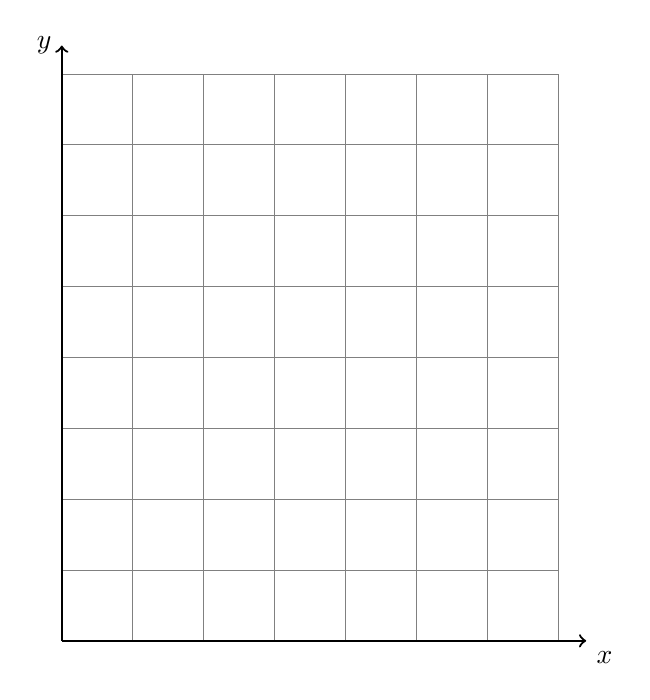
\begin{tikzpicture}[scale=0.9]
      \draw [help lines] (0,0) grid (7,8);
      \draw [thick, ->] (0,0) -- (7.4,0) node [below right] {$x$};
      \draw [thick, ->] (0,0)--(0,8.4) node [left] {$y$};
    \end{tikzpicture}
  \end{center}
  \end{multicols}
  \item Find the measure of angle $\hat{A}$.
  \end{enumerate} \vspace{1cm}

\item Given $\triangle ABC$ with $AC=9$ centimeters, altitude $h=7$ cm, and the base $AB=13 \frac{1}{2}$ cm. (diagram not to scale)
\begin{multicols}{2}
  \begin{enumerate}
    \item Write down $\sin A$.
    \item Find the measure of angle $\hat{A}$.
    \item Find the area of $\triangle ABC$. 
  \end{enumerate}
  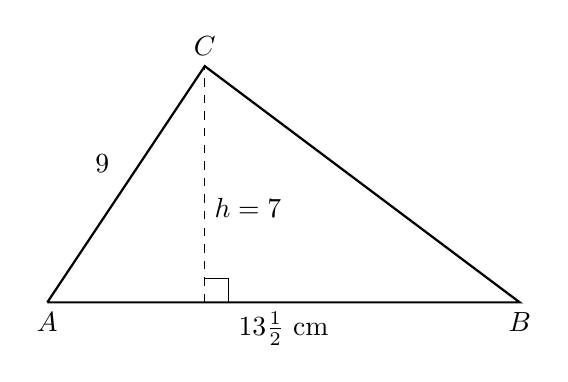
\begin{tikzpicture}[scale=1.]
    \draw [thick]
      (2,0)node[below]{$A$}--
      (8,0)node[below]{$B$}--
      (4,3)node[above]{$C$} --(2,0);
   \draw [dashed] (4,0)--(4,3);
   \draw (4,0)++(0.3,0)--++(0,0.3)--+(-0.3,0);
   \node at (4,1.2)[right]{$h=7$};
   \node at (2.7,2)[below]{$9$};
   \node at (5,0)[below]{$13 \frac{1}{2}$ cm};
  \end{tikzpicture}  
\end{multicols}
\vspace{1cm}

\newpage
\item $\triangle ABC$ is shown with $m\angle C=90^\circ$ and the lengths of the triangle's sides are $AC=6$, $BC=9$.  \hfill (not drawn to scale)
  \begin{multicols}{2}
    \begin{enumerate}
      \item Write down the value of $\tan A$. \vspace{1.25cm}
      \item Find the measure of $\angle A$. \vspace{1cm}
      \item Write down the value of $\tan B$. \vspace{1.25cm}
      \item Find the measure of $\angle B$. \vspace{1cm}
    \end{enumerate}
    \begin{flushright}
    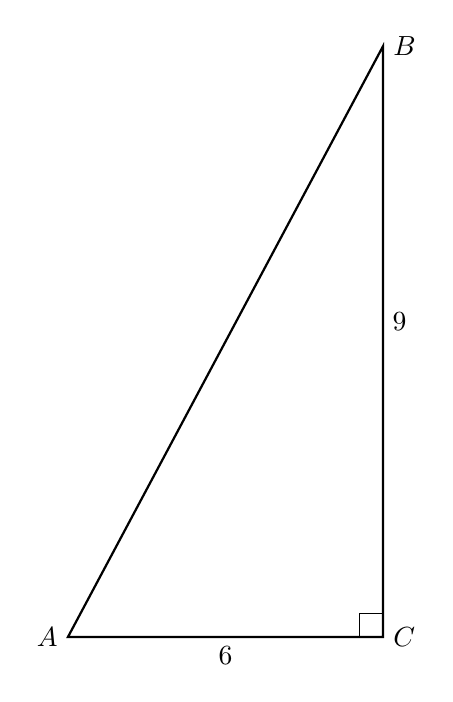
\begin{tikzpicture}[scale=0.5]
      \draw [thick]
      (0,0)node[left]{$A$}--
      (8,0)node[ right]{$C$}--
      (8,15)node[right]{$B$}--cycle;
      \draw (8,0)++(-0.6,0)--++(0,0.6)--+(0.6,0);
      \node at (4,0)[below]{$6$};
      \node at (8,8)[right]{$9$};
      %\node at (2.5,6)[above]{$17$};
    \end{tikzpicture}
    \end{flushright}
  \end{multicols}
  \vspace{2cm}
  

\item From the top of a hill a dog is visible at an angle of depression of $34^\circ$. If the hill is 11 meters tall, determine the distance from the dog to the base of the hill, \emph{x}, to the \emph{nearest meter}.
\begin{flushright}
    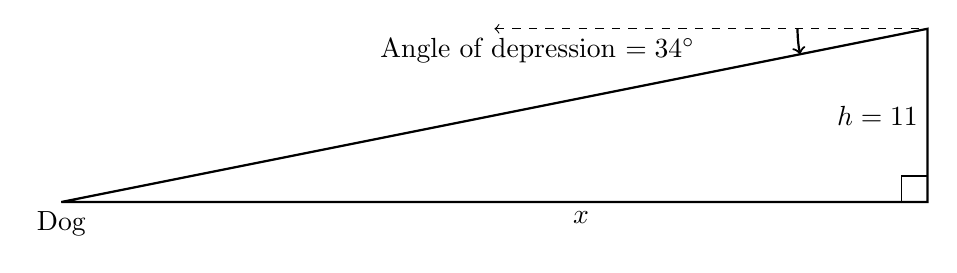
\begin{tikzpicture}[scale=1.1]
      \draw [thick] (10,0)--(0,0)--(10,2.0)--cycle;
      \draw (10,0)++(-0.3,0)--++(0,0.3)--+(0.3,0);
      \draw [dashed, <-] (5,2)--(10,2.0);
      \draw [thick, ->] (8.5,2) arc [start angle=180, end angle=191.3, radius=1.5];
      \node at (5.5,2)[below]{Angle of depression $=34^\circ$};
      \node at (10,1)[left]{$h=11$};
      \node at (6,0)[below]{$x$};
      \node at (0,0)[below]{Dog};
    \end{tikzpicture}
  \end{flushright} \vspace{4cm}
  
\newpage
\item Triangle $ABC$ has $\hat{A}=40^\circ$, $AB=7 \text{ cm}$, $BC=6 \text{ cm}$. Find the measure of $\hat{C}$.
  \begin{enumerate}[itemsep=3cm]
        \item Write down the law of sines, substituting appropriate values.
        \item Solve for the measure of angle $C$
  \end{enumerate}
  \begin{flushright}
  \begin{tikzpicture}[scale=0.6]
  \draw (0,0) node[anchor=north]{$A$}
    -- (12,0) node[anchor=north]{$C$}
    -- (6.75,6) node[anchor=south]{$B$}
    -- cycle;
    %(0,3) node[anchor=south]{$40^\circ$};
    %\draw [dashed] (1.5,0) -- (1.5,4.2);
  \end{tikzpicture}
  \end{flushright}\vspace{2cm}

\item The right $\triangle ABC$ has a base of $AC=6$ units. The area of the triangle is 15 square units. Find the lengths of all three sides and measures of all angles of the triangle. (``solve the triangle'')
  \begin{flushright}
    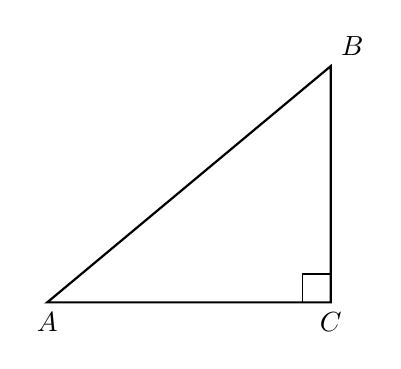
\begin{tikzpicture}[scale=0.6]
      \draw [thick](0,0) node[below]{$A$}--
      (6,0) node[below]{$C$}--
      (6,5) node[above right]{$B$}--cycle;
      \draw (6,0)++(-0.6,0)--++(0,0.6)--+(0.6,0);
    \end{tikzpicture}
  \end{flushright}
 


\end{enumerate}
\end{document}
